\documentclass{article}
\usepackage[utf8]{inputenc}
\usepackage{datetime}
\usepackage{enumerate}
\usepackage{textcomp}
\usepackage{amsmath}
\usepackage{amssymb}
\usepackage[edges]{forest}
\usepackage{tikz}
\usetikzlibrary{shapes, backgrounds, automata, positioning, arrows}
\usetikzlibrary{arrows}
\usepackage{listings}
\usetikzlibrary{graphs}

\usepackage{titlesec}
\newcommand{\sectionbreak}{\clearpage}

\title{HW3}
\author{Xinhao Luo}
\date{\today}

\begin{document}

\maketitle

\section{DPV Problem 4.11}

\textbf{Algorithm}

\begin{enumerate}[Step 1]
    \item Initialize an adjacent matrix for each element in the graph
    \item for each node n in the graph, run a Dijsktra Shortest Path to each node k in store distance to list at (n, k) (Initialize default distance to $\infty$)
    \item Initialize a temp variable \underline{min\_dist} to $\infty$
    \item Loop through each element in the matrix above the diagonal, and sum with its corresponded symmetric value of the matrix diagonal, and update \underline{min\_dist} if the sum is smaller than current \underline{min\_dist}
    \item Return no if the \underline{min\_dist} is $\infty$, else \underline{min\_dist} is the required target value
\end{enumerate}

\textbf{Runtime}

\begin{enumerate}[Step 1]
    \item initialize size will be $O(v^2)$, where v is the number of element in the graph
    \item Dijsktra Algorithm will take $O(v^2)$, as describe in lecture, and we will need to loop through each node with the algorithm, so we have $O(v^3)$
    \item O(1)
    \item Loop will be $O(v^2)$
    \item O(1)
    \item [Conclusion] The largest component of the time complexity is $O(v^3)$, so the overall time complexity of the algorithm is $O(v^3)$
\end{enumerate}

\section{DPV Problem 4.13}
\begin{enumerate}[a)]
    \item 
        \textbf{Algorithm}
        \begin{enumerate}[Step 1]
            \item For all edge e, disconnect all path that has length larger than L, the limitation of the car capacity
            \item Start from node s, do an DFS, and stop if node t is reached, and return true
            \item Return false if DFS is finish and node t is not found in when search
        \end{enumerate}
        \textbf{Runtime}
        \begin{enumerate}[Step 1]
            \item $O(|E|)$ for iterating through the graph and disconnect them
            \item $O(|E| + |V|)$ for DFS
            \item O(1)
            \item [Conclusion] Overall time complexity is $O(|E| + |V|)$, a linear solution
        \end{enumerate}
    \item 
        \textbf{Algorithm} 
        \begin{enumerate}[Step 1]
             \item Start from point s, do an Dijsktra from node s, initialize distance as $-1$. \\
             Change the update algorithm: Each time we decrease the distance from node u to v, we keep the $fuel(v) = max(fuel(u), len(u, v))$.
             \item node t's distance will be the minimum $L$.
        \end{enumerate}
        \textbf{Runtime}
        \begin{enumerate}[Step 1]
            \item $O((|E| + |V|) \times log(|V|))$ for Dijsktra Algorithm, using set implementation for findMinimum.
            \item O(1) for return value
            \item [Conclusion] Overall time complexity is $O((|E| + |V|) \times log(|V|))$
        \end{enumerate}
\end{enumerate}

\section{DPV Problem 4.20}
\textbf{Algorithm}
\begin{enumerate}[Step 1]
    \item Do Dijsktra from node s and t, save for later usage.
    \item Set \underline{result} as the distance shortest distance from s to t; Node \underline{a = s, b = t} as the final result
    \item For each edge e' from available edges, add the edge(u, v) to the graph. Calculate distance from $total\_distance = dist(s, u) + len(edge) + dist(v, t)$, while $dist(v, t)$ is the same as $dist(t, v)$ as the it is an undirected graph. \\
    If the \underline{total\_distance} is smaller than \underline{result}, let $result = total\_distance$, and node $a = u, b = v$
    \item After the iteration, check node a, b. If \underline{a == s, b == t} then there is no better solution, otherwise the path should be set between node a, b
\end{enumerate}

\textbf{Runtime}
\begin{enumerate}[Step 1]
    \item Dijesktra's time complexity is $O((|V| + |E|) * log(|V|))$, using Set implementation
    \item O(1) for initialize value
    \item $O(|E'|)$ for the for loop
    \item $O(1)$ for return value
    \item [Conclusion] The overal time complextity is $O((|V| + |E|) * log(|V|))$
\end{enumerate}

\section{DPV Problem 5.5}
\begin{enumerate}[a)]
    \item The minimum spanning tree will not change. \\
        \textbf{Prove by Contradiction}
        \begin{itemize}
            \item Assume we have mst2, after +1 for all edge, and mst1 for the original graph; and mst2 is different from  mst1.
            \item Define cost() as the sum of the total weighted edge of the graph.
            \item We have $cost(mst1) + (|v| - 1) > cost(mst2)$ 
            \item However, based on equation above, we also have: $cost(mst1) > cost(mst2) - (|v| - 1)$. This means that before the +1 for all edge, mst2 is a better solution for the graph than mst1, which is \textbf{fishy}
            \item the tree will not change.
        \end{itemize}
    \item The shortest path subject to change. Here is an example \\
        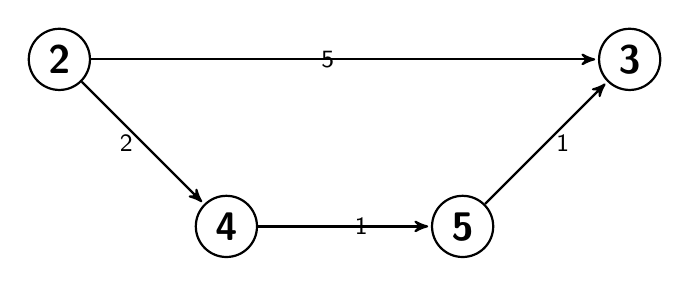
\begin{tikzpicture}[->,>=stealth',shorten >=1pt,auto,node distance=3cm,
                        thick,main node/.style={circle,draw,font=\sffamily\Large\bfseries}]
    
          \node[main node] (2) {2};
          \node[main node] (4) [below right of=2] {4};
          \node[main node] (5) [right of=4] {5};
          \node[main node] (3) [above right of=5] {3};
        
          \path[every node/.style={font=\sffamily\small}]
           (2) edge node [left] {2} (4)
           (4) edge node [right] {1} (5)
           (5) edge node [right] {1} (3)
           (2) edge node [left] {5} (3);
       \end{tikzpicture}
\end{enumerate}

\section{DPV Problem 5.6}
\textbf{Prove by Contraction}

\begin{enumerate}
    \item Assume there are two different mst(mst1, mst2) for the distinct tree
    \item Since mst1 is different from mst2, we know there must be at least one edge different between mst1 and mst2
    \item Define cost() collect the sum of the mst
    \item since each edge in the graph distinct, we have cost(mst1) != cost(mst2)
    \item Then it must be that mst1 is either better or worse than mst2, which makes one of them not qualify for being an mst. This conclusion is \textbf{fishy}
    \item There is only one mst for undirected weighted graph which all edges are unique 
\end{enumerate}
\end{document}
